\chapter{Polimorfismo}

Un método polimórfico es aquel que tiene un comportamiento diferente dependiendo del contexto en el que se realiza la llamada.

Es decir, es un método que ha sido redefinido en varias clases dependiend del uso que le queramos dar.

Tenemos un polimorfísmo en tiempo de compilación, polimorfísmo de ejecución y polimorfísmo paramétrico.

\section{Polimorfismo en tiempo de compilación}
Lo encontramos en la \textbf{sobrecarga de operadores} y en la \textbf{programación genérica} al hacer uso de \textit{templates}.

En la sobrecarga cambia el contexto mediante la lista de parámetros que recibe el método.
\begin{itemize}
	\item \textbf{Conversiones estándar} → Se convierte un tipo de dato a otro completamente diferente, por ejemplo de \texttt{int} a \texttt{double}.
	\begin{itemize}
		\item Encontramos las promociones donde se convierte un tipo a uno con mayor rango (siempre del mismo tipo), por ejemplo de \texttt{int} a \texttt{long}, pero no un \texttt{int} a \texttt{double}. 
	\end{itemize}	
	\item \textbf{Conversiones definidas por el usuario} → Se define mediante constructores de conversión y operadores de conversión, preferiblemente el segundo. Solo intenta una conversión implícita, si se puede realizar bien, si no lanzará un error.
	\item \textbf{Coincidencia con elipsis} → Si la lista de parámetros la terminamos con puntos suspensivos (…). 
\end{itemize}
En las plantillas el compilador mira los tipos de los parámetros que recibe la clase.

\section{Polimorfismo en tiempo de ejecución}
\begin{figure}[h]
	\begin{center}
		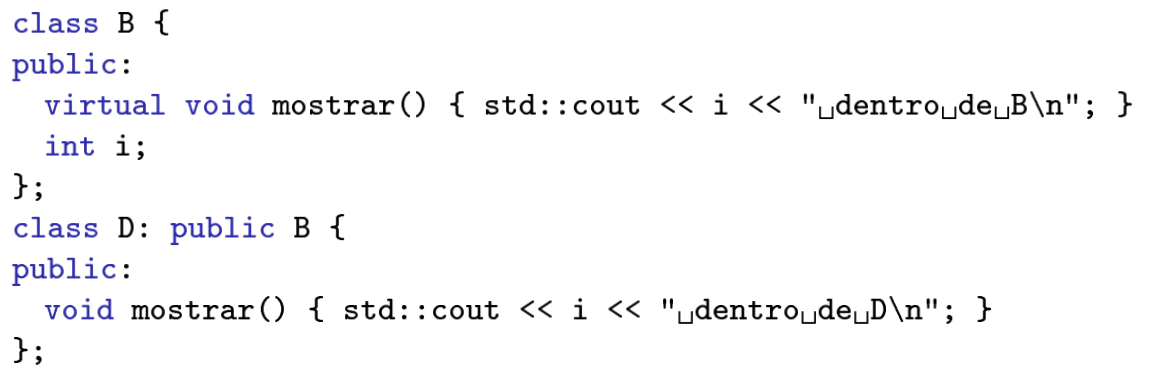
\includegraphics[width=\textwidth]{Imagenes/pol1.png}
	\end{center}
\end{figure}
La clase B es una clase \textbf{polimorfica} ya que tiene un método definido como \texttt virtual}.

La clase D tendrá dos miembros → el atributo \texttt{int i} y el método \texttt{mostrar()} , ya que hemos definido el método `\texttt{mostrar()} ) de la clase B como virtual, es decir el compilador sabe que ese método es polimórfico y por tanto se redefinirla en la clase derivada.

Esto sucede siempre y cuando la clase derivada tendrá un método con el mismo nombre y ese se defina como `virtual` en la clase base.
\begin{figure}[h]
	\begin{center}
		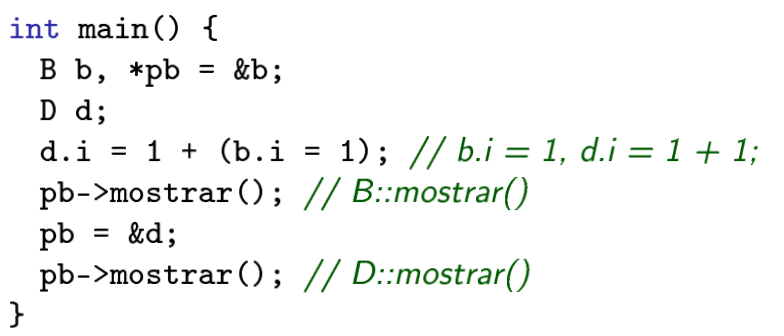
\includegraphics[width=\textwidth]{Imagenes/pol2.png}
	\end{center}
\end{figure}
